%\addcontentsline{toc}{chapter}{Development Process}
\chapter{Design}

%You should concentrate on the more important aspects of the design. It is essential that an overview is presented before going into detail. As well as describing the design adopted it must also explain what other designs were considered and why they were rejected.

%The design should describe what you expected to do, and might also explain areas that you had to revise after some investigation.

%Typically, for an object-oriented design, the discussion will focus on the choice of objects and classes and the allocation of methods to classes. The use made of reusable components should be described and their source referenced. Particularly important decisions concerning data structures usually affect the architecture of a system and so should be described here.

%How much material you include on detailed design and implementation will depend very much on the nature of the project. It should not be padded out. Think about the significant aspects of your system. For example, describe the design of the user interface if it is a critical aspect of your system, or provide detail about methods and data structures that are not trivial. Do not spend time on long lists of trivial items and repetitive descriptions. If in doubt about what is appropriate, speak to your supervisor.

%You should also identify any support tools that you used. You should discuss your choice of implementation tools - programming language, compilers, database management system, program development environment, etc.

%Some example sub-sections may be as follows, but the specific sections are for you to define.

As the application was developed in an iterative manner, over a series of sprints, class diagrams and design diagrams were not created at the very start of the project. Over a series of sprints designs were iteratively developed regarding the system overview. However, some design decisions were decided at the start of the project. The chapter will clearly explain rationale for the decisions and state whether the design decisions were a result of iterative processes or upfront design.

\section{Implementation tools}
The following discusses the design decisions regarding the implementation tools that were used during the project, providing rationale for the choice of tools.
\subsection{Programming language}
With the programming language choice unlikely to change per sprint, then an upfront design decision was made. From the analysis it was concluded that the application would be implemented as a web application.  A consideration between different server side programming languages was considered in depth.

Typically with server side applications the traditional language choices are: PHP, Ruby, Python, C\#, Java and JavaScript, which has increased in popularity recently \cite{citeulike:14018462}.

Evaluating the analysis decomposition in the meetings in the beginning sprints it was determined that OpenCV, would be needed to be utilised in the project. OpenCV's original source code is written in C++, however Python and Java bindings to OpenCV are available. Additional research was conducted to see if a reliable wrapper for either PHP or Ruby was available, and after a lot of investigation it was concluded there was not.

C++ is not considered a standard web application development language, therefore reducing the opportunity for support during the project, it was dismissed as viable choice. Java applications are predominately large commercial applications, using a range of enterprise software - often renowned for their performance abilities \cite{citeulike:14019744}. This approach felt too cumbersome for a proposed light-weight application.

By being constrained by design decision to use OpenCV coupled with the lack of reliable wrappers for other languages and a reluctance to use Java then Python was selected as the most suitable language. Python offers a lightweight and quick to learn syntax that produces readable code whilst allowing a object-oriented paradigm to be followed. Additionally, its support for OpenCV is sufficient for the application.


\subsection{Choice of framework}
To recap, Python was chosen as the language of choice for the application. Frameworks aid in the development of a project, especially with web applications where routing is often required; often routing support is a key feature of frameworks. Exploratory work was completed in the early sprints to find a suitable tool. The frameworks Django \cite{citeulike:14019784}, Flask \cite{citeulike:13160396} and Bottle \cite{citeulike:14019792} were evaluated.

Some frameworks constrain the developer's to specific implementations through abstracted classes whereas some offer more flexibility. Whilst evaluating Django, a full framework, it was concluded that such a large framework was excessive for this application and rejected as a choice for the framework.

Flask and Bottle are classified as ``micro-frameworks'', offering a lot less restrictive structure and allowing the developers to have more control on how the applications are structured. On face value, Flask and Bottle appear to be very similar: they are both lightweight with a similar syntax. Evaluating both of the frameworks identified that Flask had a larger support community than Flask, coupled with better documentation, compared to Bottle. As neither framework had been used before then a support community was an important design decision.

As a result, Flask was chosen as the framework which will be used throughout the application. Spike work was completed to see how simple it was to create a quick application, after discovering it was perfectly fine, Flask was agreed as the framework of choice.

\subsection{Database management system}
As the analysis suggested it should be a web application then data persistence should be an integral part of the application. Prior to choosing an appropriate tool, a rationalised decision had to be made on the different management systems available.

\subsubsection{NoSQL or relational database management systems}
The choice of database management system was considered at length. Firstly, the decision of whether to use NoSQL or a relational database management system (RDBMS) had to be decided. This was decided during the early sprints, whilst the design was beginning to emerge.

RDBMS's are suited to separating the data into logical relations which decouples through the process of normalisation. The data normally suited to a RDBMS is one which has a uniform structure and can be represented as a series of relations, with specific constraints.

NoSQL provides a more flexible structure, allowing data to have no specific structure. In MongoDB \cite{citeulike:14019766} documents are equivalent to relations - structuring the data as key-valued pairs over specific column structures. This offers more flexibility in the data passed to the database.

From previous design choices made in prior sprints regarding the database structure, both options were seriously considered. After the analysis of what the note meta data would consist of, it was decided that the structure for the data would not vary, each note will have an associated lecturer, title etc, then a relational database would be suitable for the application. In addition, the notes \textit{must} follow a specific layout structure, therefore affirming that data would be linked and structured.

A specific choice of RDBMS had to be chosen as an appropriate tool to persist the data from a note; digital ocean offered a concise comparison aiding in the design \cite{citeulike:14019772}.
\subsubsection{SQLLite}
SQLLite was considered as a viable option; Flask provides documentation for its ease of use with the micro-framework. Considering the larger picture: would it scale well with multiple users interacting with it? Digital ocean state it would be a perfectly fine testing and development tool, but for production it may not scale well with multiple reads and writes.
\subsubsection{PostgreSQL}
Digital ocean describe PostgreSQL as the most advanced of the RDBMS's available. The additional support of more types an attribute can have allows for a greater control when creating a database. For example, the JSON type support would allow the application to save returned JSON from 3rd party services directly to the database.
\subsubsection{MySQL}
MySQL and PostgreSQL for most applications would be interchangeable. It offers a wide range of support along with comprehensive documentation. There are concerns over performance, however.

\noindent
After evaluating the possible RDBMS's it was concluded that MySQL and PostgresSQL would be more preferable for scalability. Although there is not a great difference between the two, PostgreSQL was chosen for its advanced ability allowing for the application to become more advanced. This goes against the YAGNI (you ain't gonna need it) approach, but infrastructure decisions are harder to change, than code implementations.

\subsection{Continuous integration tools}
Continuous Integration (CI) is normally used in development teams to ensure that all code is checked into the repository. For the single person project it was adapted. The value was not to ensure all code was checked into the repository, but to build the project on each individual branch to ensure every commit passes associated tests written.

Since CI was decided to be used in the analysis stage, a specific tool in aiding in CI would have to be chosen. Jenkins was an initial choice; it is a standalone Java application which a repository can be synced to.

Another option was Travis CI, a CI tool in the cloud which can be attached to a GitHub repository. It runs tests on every commit to a repository if there is a travis.yml file committed. Travis then build the application and reports whether it errors, passed all the tests or failed any tests.

A key design decision was to be able to check the build process quickly. With Travis it has a web interface clearly showing the output. Jenkins would require additional set up of specific build scripts for every branch in the application. Therefore, Travis was chosen for the ease of use and a nice integration with the repository.

\subsection{Version control}
Version control was utilised on the project to ensure that code was continuously added, allowing the option to revert changes if necessary. The project was created on a private Git repository on GitHub. Git was chosen for its familiarity and GitHub is a well known place for handling versions of software. Github also tied in well with other tools such as Travis CI.

\section{Overall Architecture}
This section discusses the architecture of the web application as a whole. The process of the design with the web application was developed over a series of sprints, rather than an upfront design.
\subsection{CRC cards}
To recap, Extreme Programming uses the concept of CRC cards to help to aid the developer to consider the design of the application. Unlike UML, they are throw-away cards which can be edited and changed every time a new feature is implemented. The CRC cards which have been drawn up in the application have been formalised.

\begin{figure}[h]
  \centering
  \includegraphics[scale=0.5]{images/CRC_card}
  \caption{An example from Sprint 3, showing a CRC card at the very beginning of creation.}
  \label{fig:crc1}
\end{figure}

Figure \ref{fig:crc1} shows an example of a CRC card at the very beginning of the note class creation. The left hand side helped to think about methods and attributes that the system must do. The right hand side shows the responsibilities, where the note may interact with other class.

These classes were then implemented into classes. This process was completed at every feature. The appendix X shows more CRC cards in the application.
\subsection{Class Diagram}
After CRC cards were produced, they can be easily transformed into formal UML in the form of a class diagram. The class diagram was collated as a retrospective of the CRC card design, and designed after the sprints. The CRC cards were used as an iterative design and now a class diagram is formalising that design decision.

Figure x in appendix x shows the class diagram.

\subsubsection{Justification of design}
The following subsection will justify design decisions from the class diagram and the behviour it intended.
\subsubsubsection{Google services}
The $BaseGoogleService$ class is a super class which has the $GoogleCalendarService$ and $GooglePlusService$ extending as sub classes of the system. Common functionality was shared between the sub classes, where queries had to be built and then executed ($execute_request$). These were moved to the superclass to remove this duplicated functionality.

Both the $GoogleCalendarService$ and $GooglePlusService$ classes have constant variables: $API$ and $VERSION$; these values are unlikely to change, but are identified as variables so they can be changed easily.

With $GoogleCalendarService$ it is expected that the class controls all integration with data which involves direct access to the Google Calendar API. Important functions include getting a list of events, returning JSON event listings from the service and adding and removing description based content.

The $GooglePlusService$ has a key function of parsing the user's email address from the response returned when they authorise with OAuth.

The $OAuthService$ class allows the user to authenticate via oAuth with the Google services. When the class is called, the procedures go through exchanging tokens and eventually authorising with Google.

\subsubsubsection{Helper classes}
Helper classes are used to aid the application from reducing amount of repeated code. Often these helpers were implemented in various controllers, so reducing the code duplicated code helped with a readable system.

The $TesseractHelper$ has a range of functions which aid with the interaction of Tesseract and the user's uploaded note. This class is instantiated when the user uploads an image.

$GoogleServicesHelper$ class was created to purely deal with duplicated code. It stores no attributes in the class and all the methods are static - this decision was made due to the duplication of similar code in multiple controllers. This class was extracted out and groups similar GoogleService calls in a similar place.

$SessionHelper$ class was created to deal and handle with the appropriate sessions in the application. Partly created to ease with testing and partly created to reduce unsemantic code in the controllers. The session helper is instantiated in every controller where sessions are being used.


\subsubsubsection{Persistance model classes}
Each of the model classes extend the SQLAlchemy model classes. The models mirror that of the database design, for the attributes, which more information can be found on sections TODO.

In the $User$ table implements a static method: $find_user_by_email_address$. This was chosen to be a static, so that the method could be called without needing a user object to exist. This groups together relative information about the user to the user model, but without the need for another object to be created. This principle is also applied to the $NoteMetaData$ for the $find_meta_data$, $Note$ class and $find_id_by_module_code$ and $Note$ class and $find_note_by_module_code$. Overall these classes implement specific save functions to encapsulate database transactions in one place.

\subsubsubsection{Other classes}
The $CalendarItem$ is called from the view file when parsing a list of events it would display the date correctly.

$InputValidator$ class is implemented to handle all the upload data from a user. It is there to check the data entered is valid from the user. It's instantiated from the add meta data routes and the edit meta-data routes. It helped to reduce the data redundancy.

A $FileUploadService$ is used to ensure that when the user uploads their file that specific constraints were met. It also allows the user to save the image to the filestore.

An $ExifParser$ was used to extract the EXIF data from an image when the user uploaded the item. A constant integer, which depicted the ``datetime'' field from the exif response was stored so that the date time from the image can be extracted.

Finally the $BinariseImage$ class, constructs all the OpenCV code for binarising a user's uploaded image into black and white. The purpose of the classes purpose discussed in section X. The class eventually saves an image to the filestore and is called from the fileupload controller.


\subsection{Database diagram}
Coupled with the CRC cards a database UML diagram has been produced which shows the implementation of the relations in the database.

\begin{figure}[h]
  \centering
  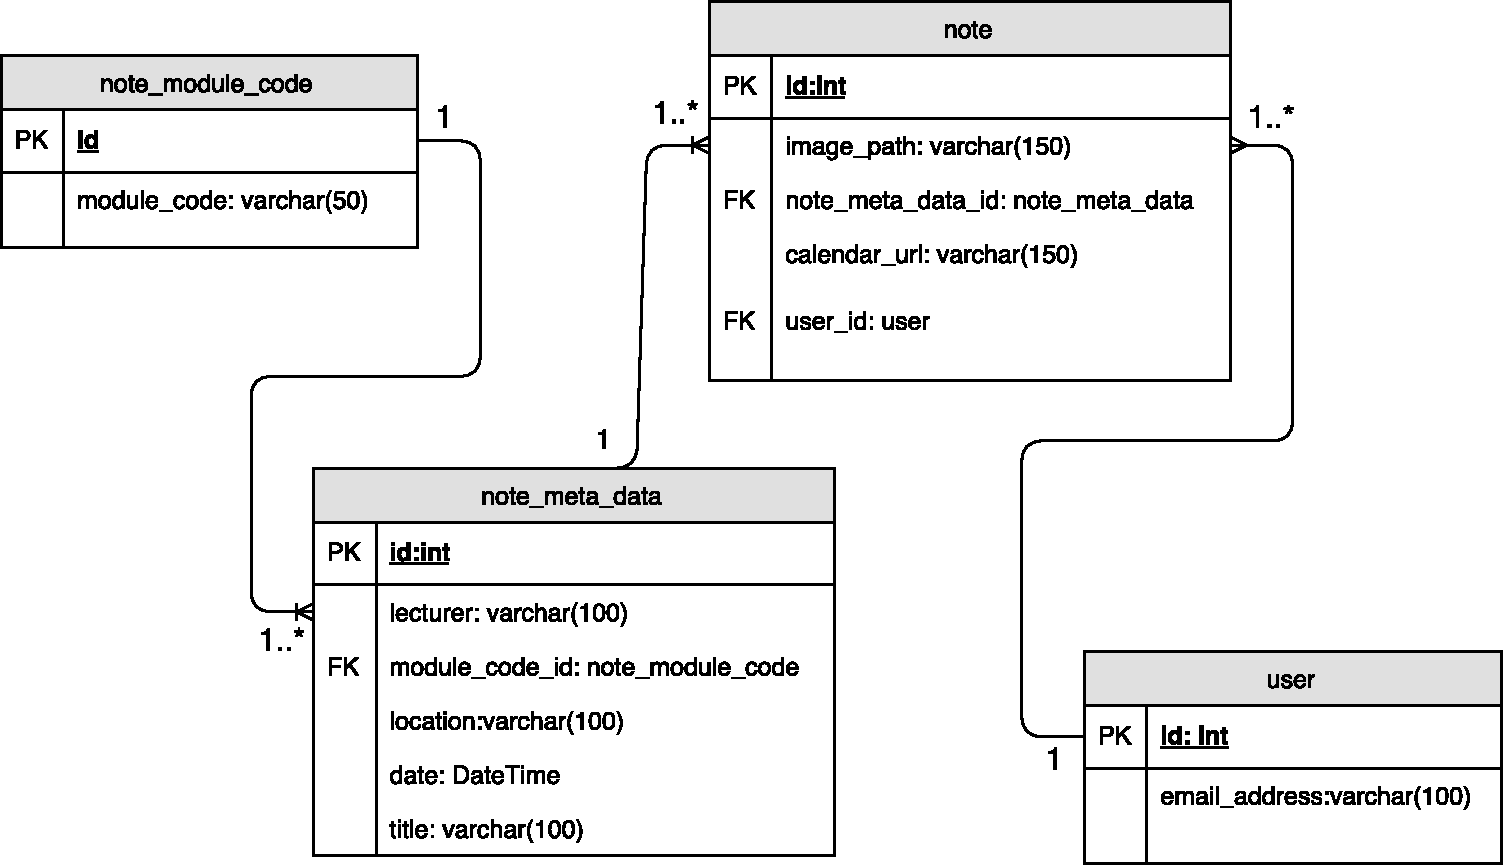
\includegraphics[scale=0.5]{images/database_diagram}
  \caption{The final result of the database diagram. After a series of iterations.}
  \label{fig:database}
\end{figure}

Figure \ref{fig:database}, shows the output from the result of continuous design on the database diagram through the iterations.

\subsubsection{Justification of design}
The design has been carefully considered. The reason the note is in its table is intuitive: a note needs to be persisted in the database. The attributes best collate a high-level representation of what a note consists of. First and foremost,  a note will consist of an image link - which is a relative path, this was stored to persist where the image on the file store is located for that image. A user id was added to the note, to link a note to a user; not originally in the scope of the application, but a design feature added so that it was more accessible.

The calendar url was added to the database to persist which calendar event was associated with the note. As a note will only have one calendar event, then saving it in the database was an easier way to link to the event - rather than making an external API request to Google.

Finally with the note relation, a note-meta-data foreign key id was added to link additional note-meta-data to a note.

The Note-meta data relation is its own relation because of reducing data-redundancy, this is a key requirement in normalisation of databases [CITE]. The note Meta-data may be duplicated in a note if a user takes more than one note per lecturer - and wants to tag the same meta-data to the note. As a result a relation was created for this use-case.

The meta-data consists of a lecturer, location, and title as variable characters up to 100 in length, which is a valid length as none of them realistically should be more than that length. A date field was added so the meta-data can be associated to a date and time - this aids in the calendar integration. Finally, the module code is identified as a foreign key constraint.

The module code is its own relation, and therefore a foreign key in the meta-data relation is because of the same reasons as meta-data is it's own relation: data redundancy. A valid use-case is that a user would enter in multiple notes for any given module code. This module code does not need to be duplicated in the database - therefore a foreign key was suitable.

Finally, a user relation was established after the application decided it would be expanded to involve users. An email address was created to parse the response from the oAuth log-in. Furthermore, this was added as a foreign key to notes, so that every user would be associated to a note.

Overall, a succinct collection of relations have been developed, which follow a good normalization process to produce a design from a database side which has been well considered.

%\section{Some detailed design}


\subsection{MVC Structure}
Early on in the process it was decided that an MVC approach would be approached. This was an upfront design decision, that would not likely to be changed.

\subsubsection{About MVC}
MVC is a design pattern where you split the logic into a Model View and controller. As displayed in figure \ref{fig:mvc} the MVC approach helps to decouple logic from the view file. Therefore all the information passed to the view is renderable content. The controllers do not integrate with the database directly. The primary job for the controllers is to interact with the model, any services and ask to render the view files.

The model in the MVC structure has no acknowledgement of the view file. Instead of rendering any form of HTML in the model it is purely data-driven. The sole purpose of the model is to interact with the database and perform any business logic that does not fit in the controller and the view file.

Finally, the view files contain HTML logic with dynamic content passed to the file from the controller. There may be specific logic which impact the HTML displayed, but no direct calls are made to the database layer or the controller. It uses the dynamic content passed in.
\begin{figure}[h]
  \centering
  \includegraphics[scale=0.5]{images/MVC}
  \caption{A example of how the model-view-controller(MVC) framework integrates.}
  \label{fig:mvc}
\end{figure}

\subsubsection{Structuring the Web application}
The application was chosen to follow the MVC approach so that there was a clear distinct design pattern used, which did not obfuscate where logic and presentation layers interact. With a well structured system it makes testing easier.

In addition to the structuring, components can be reused again easily. Take for example service classes, these are reusable components in the system where they can be easily instantiated from inside any controller. If an MVC approach was suggested for the design then the reusability of code would decrease. This could only be achieved from a nice decoupled system where independent logic can be processed separately.

Although the MVC approach was desired, Flask does not support an MVC structure out of the box. During a lot the documentation it expects all routes to be placed in a single file. This design approach was not considered for a number of reasons: it reduces the readability of the code - if there is more than one class per file, then readability begins to be impacted. Furthermore, when considering the design of the controller objects, as well as the models, then dependencies between the classes would become obfuscated. From identifying an architecture perspective, if the routes were on one file and models in another, it would be hard to explicitly identify corresponding links between different files.

To overcome the Flask routing issue, in recent versions [FIND VERSION NUMBER] Blueprints [CITE] have been included. These blueprints, act almost as controller files, like Ruby, using the routing annotation to create a route. Therefore, similar routes can be place in the same file, but a different file can be created for unrelated routes. This offers a good controller feel to the application.

The models consist of both persistence logic as well as service and helper objects. All the business logic is kept in side this group. Finally, all the views are allocated to the view directory.

\subsubsection{Extending views}
It is worth mentioning that Flask uses the Jinga templating engine[CITE]. By default Jinga would expect the DOM to be represented again in every view file. A design decision was made to extend the view files. Figure \ref{fig:extension} illustrates the view file design.
\begin{figure}[h]
  \centering
  \includegraphics[scale=0.5]{images/view_file_extension}
  \caption{A diagram illustrating how extension in Jinga html template engine works.}
  \label{fig:extension}
\end{figure}

Each of the view file templates are separated into their own directories. Inside the directories, the HTML files extend the index.html root file. This overrides the block ``content'', dynamically generating a new content for every new URL. The advantages of this design is that meta-data, headers, stylesheets and navigation can be placed in the index.html page and all subpages will inherit these automatically, sticking to the principle of DRY.

\subsection{Application URLs}
When considering the application URLs would form an integral part of helping the users to identify where they are, what the page is aiming to achieve and, where applicable, bookmarkable.

Therefore designs into the URL structure was performed. Typically there are two types of URL structures which websites take: query strings or REST URLs.

Query strings aid in the creation of URLs such as: /search?name=foo. The query string is represented as a key value pairing of the searched criteria. This form of URL representation is acceptable for search criteria, but what if the user was editing a note - would a good structure contain all the contents of that note?

For parts of the application to overcome this issue REST [CITE] URLs were considered. By exposing the URLs to RESTful interface, it is clear what the application is intending to do on that page. For example $/show_note/1$ compared to $/show_note?note_id=1$. Therefore, the URLS will follow a hierarchal structure, showing exactly where the notes are, in this case [CITE].

It is worth noting that RESTful URLS are a good concept for external API usage. However, due to the application being a web application some modifications were taken place. For example, the URL: $/view_notes/$ would be a better RESTful url as /notes/. However, the design decision was to adopt the RESTful pattern to help make the URLs a bit more readable, but still keep the principles of REST.

\subsection{HTTP methods}
Flask supports all the REST HTTP methods, such as delete, put and patch[CITE]. However, normal web browsers have this common issue where they do not support them and instead only support GET and POST.

As a comparison in Ruby, the templating language - embedded ruby - allows being able to fake certain methods on forms and submit buttons. Unlike Flask, who uses pure HTML templates, with the Jinga syntax added on top, then developers are restricted to the default GET and POST.

Another layer of code could have been added in the form of posting everything to the URL routes on the server as AJAX requests - but that would first and foremost change the entire structure of the application. This would mean that a user would have to have Javascript enabled on the page to even interact with the application.

As a result, the design decision to use default POST and GET requests was decided. DELETE would not be used for deleting content from the database.

\subsection{Interaction with the application}
When decomposing a problem it is useful to identify how a user would intend to interact with the system.





\section{User Interface}
Although the application was developed in an iterative approach, wiremocks were completed when UI changes occurred so that I could reflect on them.

To begin with the user interface (UI) went through a few iterations of wiremocks to sketch out what it should look like.  This iterative approach was applied when actually designing the website. Firstly it was important that the application felt as thought it was an application, rather than a traditional website. Colours from Google Style guide [CITE] was used to keep with nice, clean and bold colours. Bootstrap[CITE] was considered to be used on the application and it did give a default responsive theme built in - however, keeping with the idea of minimalist and not over-bloated, then personally I feel that that bootstrap comes with a lot of the additional material which would not be needed.

With this being a web application, a responsive navigation was always important. A user may take a photo of their note and then upload this to the website off their mobile. This resulted in the web application having to be thought about from a responsive view. I should have done this better and considered this from the beginning and built up from the responsive to the desktop version. However, I did retrospective responsive design and performed media-queries when I needed to.
% add in code examples for media query\
\begin{itemize}
  \item Wiremock examples
  \item Media query code examples.
\end{itemize}
% Include wiremocks
\section{Other relevant sections}

\begin{itemize}
  \item Why Parsing the notes returned the first 3 lines. Why did this have to be done?

\end{itemize}

\subsection{Tesseract}
Comparisons between different OCR tools was researched. Evaluations into systems which would be a suitable aid was undertaken. [CITE - Case study] performs a case study using Tesseract as their OCR tool to analyse printed text in an image. Patel et al, also discuss the comparison against a proprietary OCR tool, Transym [CITE].

The results concluded by Patel et al is that Transym only yielded a 47\% accuracy on 20 images compared to 70\% accuracy using the Tesseract engine.

Analysing the outputs concluded that Tesseract would be the best performing on an image. Tesseract was chosen for its open source and it's highly commended recognition rate as well as my supervisor echoing the compliments of Tesseract and it should be considered.

\section{Optimising tesseract}

\subsection{ImageMagick}
Once Tesseract was chosen as the OCR tool training was started promptly. Due to there not being a formal way images were supposed to be prepared for the tool then the first few iterations were converted to grayscale using ImageMagick [CITE]. This yielded a poor return rate and characters were not identified consistently.

At this point in the design, the notes were being written on original lined paper. Research work was looked into to try and get the image as clean as it could be for the Tesseract engine. This resulted in monochrome from ImageMagick to be used; an increase in recognition rate was received, however the image was very messy with pixels from the lines obfuscating the response from Tesseract.

\subsection{OpenCV}
During a meeting with Dr Hannah Dee, it was suggested that OpenCV should be used. It was already a design consideration - as to why Python was chose - so it should be used to facilitate the binarisation script.

OpenCV is an open source image processing library. Natively written in C++, but there are Python bindings available - so the Python version was selected, to fit into the web application.





\begin{itemize}
  \item Realised it wasnt good so redesigned it to custom lined paper Why did I do this instead of normal lined paper?
  \item Why the colour blue ?
\end{itemize}
